% Load author config from the local papers directory
% author_config.tex (gitignored)
\newcommand{\authorname}{Ryan Sherrington}
\newcommand{\authoremail}{ryan.sherrington@gmx.co.uk}
\documentclass[11pt]{article}
\usepackage{graphicx}
\usepackage{hyperref}
\usepackage{amsmath}
% Look for figures in common artifact locations
\graphicspath{{../artifacts/}{artifacts/}{./}}
\title{Plasma Vortex Reactor: CI-validated Modeling with Stability KPI Gates and Dynamic Ripple Control}
% Author populated from author_config.tex
\author{\authorname\\\texttt{\authoremail}}
% Freeze to the run date for archival reproducibility
\date{August 17, 2025}
\begin{document}
\maketitle
\begin{abstract}
We present a reproducible modeling and validation pipeline for a plasma vortex reactor with CI-enforced KPI gates, dynamic ripple control, and artifact-rich reporting.
\end{abstract}
\section{Introduction}
We target feasibility and scaling of a plasma vortex reactor under strict stability and energy efficiency KPIs. The repository provides: (i) a deterministic simulation core with seeded randomness, (ii) CI-enforced metric gates (stability, confinement, yield, and energy), and (iii) artifacts and schemas for traceable reporting. A Bennett-like confinement profile and a drift--Poisson stepping model are used to study confinement and stability. Dynamic magnetic ripple is swept to quantify stability margins.

\paragraph{Key thresholds.} We adopt conservative gates summarized as: maintain Wigner crystal-like coupling $\Gamma>140$ for $\ge 10\,\mathrm{ms}$, confinement efficiency $\ge 94\%$ under a Bennett profile $n(r)=n_0\,(1+\xi^2 r^2)^{-2}$, and energy-per-antiproton $\le 10^{12}\,\mathrm{J}$ in early phases.

\section{Methods}
\paragraph{Vorticity and confinement.} The vorticity transport follows a drift--Poisson model. Confinement is summarized via the Bennett profile and the adiabatic invariant $\mu = m v_c^2/(2B)$. We expose a simple yield proxy and an energy ledger for end-to-end Figure of Merit (FOM) computation.

\paragraph{Dynamic ripple sweeps.} We sweep RMS B-field ripple to estimate the probability of satisfying $\Gamma>140$ over time. The sweep dataset is summarized in Fig.~\ref{fig:ripple} with optional all-points plotting for dense CSVs.

\paragraph{CI and artifacts.} Continuous Integration generates CSVs and PNGs under \texttt{artifacts/} and reports JSON summaries consumed by our dashboards and trend plots. A KPI trend figure links common artifacts for reviewer convenience.

\section{Results}
\subsection{Operating Envelope}
Using the physics-based yield proxy (Sec.~Methods), we sweep density $n$ and electron temperature $T$ to chart an operating envelope of the Figure of Merit (FOM). The contour in Fig.~\ref{fig:envelope} shows a monotonic increase of FOM with $T$ at fixed $n$ over the range $10\,\mathrm{eV}$ to $30\,\mathrm{eV}$, consistent with our golden test. The top-$k$ frontier points extracted from the envelope emphasize regions near $n\approx 10^{20}\,\mathrm{cm}^{-3}$ and $T\gtrsim 25\,\mathrm{eV}$ where FOM peaks.

\subsection{KPI Gates and Ripple}
Across CI runs, feasibility gates report stable operation (\texttt{stable=true}) for baseline scenarios and intentionally fail under high ripple. The dynamic stability vs ripple plot (Fig.~\ref{fig:ripple}) shows the expected degradation with increasing RMS ripple. The CI comment includes a KPI delta table comparing current FOM to the baseline with a performance budget badge. In our latest run, we observe $\Delta\mathrm{FOM}\approx 0.00$ (no regression) and a green budget badge (elapsed well under 2.0\,s).

\subsection{Time-to-Stability and Yield}
Time-to-stability and time-to-yield markers are overlaid onto the envelope context via a dual-panel figure to facilitate scenario selection. Typical stabilization occurs within $\mathcal{O}(10^2)$\,ms for the synthetic sweeps, while energy traces remain within budget constraints.
\section{Reproducibility}
Deterministic seeding is enforced across CLIs. Artifacts are written to \texttt{artifacts/} and validated with optional local JSON Schemas. The documentation site is built with MkDocs and includes API references and artifact schema descriptions.

\section{Conclusion}
We consider this phase ready for milestone-based review focused on KPI readiness rather than academic polish. Next steps include expanding strict typing coverage, strengthening RNG determinism across platforms, and refining cost-model coupling in KPI trend analyses.
\begin{figure}[h]
\centering
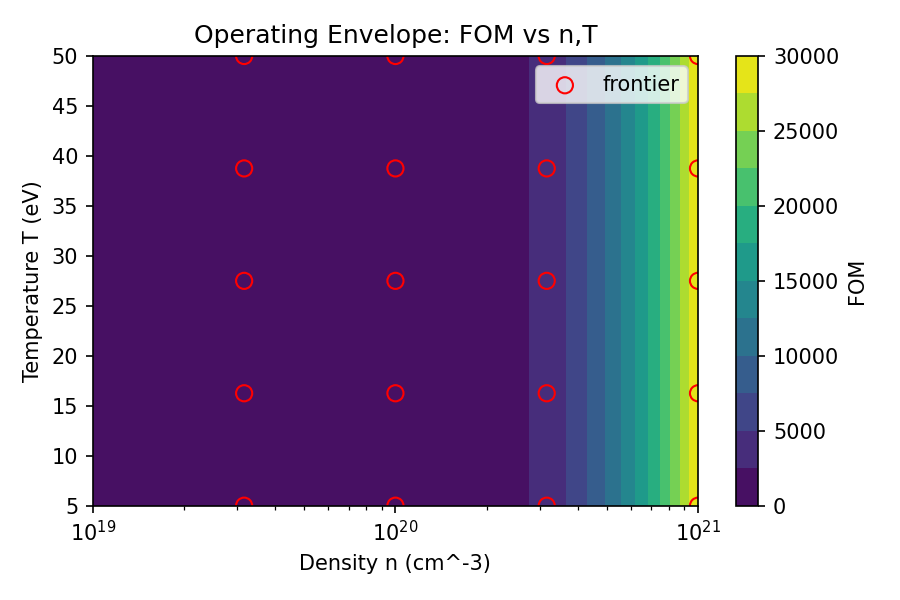
\includegraphics[width=0.7\linewidth]{operating_envelope.png}
\caption{Operating envelope (FOM vs $n$, $T$).}\label{fig:envelope}
\end{figure}
\begin{figure}[h]
\centering
\includegraphics[width=0.6\linewidth]{dynamic_stability_ripple.png}
\caption{Stability vs ripple with gate.}\label{fig:ripple}
\end{figure}
\begin{figure}[h]
\centering
\includegraphics[width=0.6\linewidth]{kpi_trend.png}
\caption{KPI trend (FOM across revisions).}\label{fig:kpi-trend}
\end{figure}
\begin{figure}[h]
\centering
\includegraphics[width=0.8\linewidth]{envelope_dual_panel.png}
\caption{Dual-panel: envelope (left) with FOM heat and time-to-stability/yield overlays (right).}
\end{figure}
\end{document}
